\documentclass[../index.tex]{subfiles}
\begin{document}

\section{Циклы}\label{sec:loops}

    Вооружившись ранее изученным набором команд, вам не составит труда реализовать цикл на динамическом языке.
    
    Напишем программу, которая выведет в поле <<Результат>> 100 точек:
    
    Добавьте  на динамическую форму скрытое поле с 'id' : 'counter'. Это поле будет служить счетчиком цикла.
    
    Ниже приведен полный листинг программы:
    
    \begin{verbatim}
    if(
        [isnotin([getValue([counter])],[100])],
        [run(
            [setValue(
                [plus(
                    [getValue([result])],
                    [.]
                )],
                [result]
            )],
            [setValue(
                [plus(
                    [getValue([counter])],
                    [1]
                )],
                [counter]
            )],
            [call(
                [getValue([cmd])],
                [this]
            )]
        )]
    )]
    \end{verbatim}
    
    Запустив программу, можно убедиться, что в поле <<Результат>> вывелось ровно 100 точек.
    
    Теперь рассмотрим принцип работы программы подробнее:
    
    \begin{verbatim}
    if(
        [isnotin([getValue([counter])],[100])],
    \end{verbatim}
    
    В данном фрагменте кода мы проверяем, не выполняется ли условие неравенства нашего счетчика значению 100.
    
    В этом случае выполняем тело цикла, состоящее из 3-x команд внутри блока <<run>>:
    
    \begin{verbatim}
    setValue([plus([getValue([result])],[.])],[result])
    \end{verbatim}
    
    Здесь происходит добавление новой точки в поле с результатом.
    
    \begin{verbatim}
    setValue([plus([getValue([counter])],[1])],[counter])
    \end{verbatim}
    
    Увеличиваем значение счетчика на 1.
    
    \begin{verbatim}
    call([getValue([cmd])],[this])
    \end{verbatim}
    
    И, главная часть, обеспечивающая зацикливание нашей программы - вызываем повторное выполнение скрипта при помощи функции
    <<Call>>
    
    \begin{figure}[h]
    	
\includegraphics[width=0.6\textwidth]{meme_visable}
    	\centering
    \end{figure}

\section{Вложенные команды}

Рассмотрим классическую задачу, встречающуюся в большинстве шаблонов динамических форм. Зачастую требуется установить ряд свойств динамического элемента, например, "выключить" и "скрыть":
\begin{verbatim}
run(
    [setVisible([false],[this])],
    [setMandatory([false],[this])],
    [setEnabled([false],[this])]
)
\end{verbatim}

Указанный фрагмент кода прекрасно справляется с поставленной задачей. Однако, скрипт можно заметно облегчить, применив технику <<Вложенных команд>>:

Обратим внимание, что каждая динамическая команда в данном примере возвращает значение -- id динамического элемента. Таким образом, мы можем передавать команды в качестве аргумента с ожидаемым значением id в другие команды. Применив данный подход
дважды, сократим код примера до следующей записи:

\begin{verbatim}
setEnabled([false],
  [setMandatory([false],
    [setVisible([false],
      [this])])])
\end{verbatim}

Мы также избавились от необходимости использования динамической команды <<run>>!

В общем случае, алгоритм рефакторинга по технике <<Вложенных команд>> выглядит так:

\begin{enumerate}
    \item В списке аргументов функции <<run>> убедитесь, что возвращаемые значения всех команд семантически совпадают с входными параметрами других команд. В большинстве случаев - это id элементов на форме.
    \item Возьмите последнюю команду из списка и замените подходящий литерал аргумента предшествующей команды ее вызовом.
    \item Удалите последнюю команду из списка.
    \item Если в списке аргументов функции <<run>> осталась одна команда -- замените блок <<run>> этой команды, иначе повторяйте шаги 2--3.
\end{enumerate}

\begin{figure}[h]
	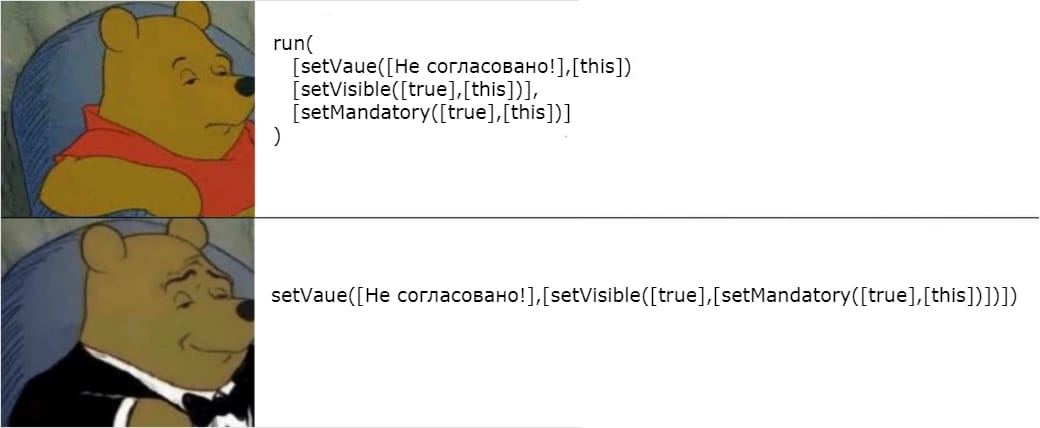
\includegraphics[width=0.8\textwidth]{meme_pooh}
	\centering
\end{figure}

Внимание! 
Избегайте злоупотреблений рассмотренным приемом -- избыточная вложенность усложняет читаемость и поддерживаемость кода: удалить или добавить команду в середину цепочки вызова становится затруднительно. Рекомендуемый уровень вложенности -- не более 3--4.
    
\section{Выделение функций}
    
Рассмотрим задачу формирования списка месяцев в зависимости от текущей даты: в элемент типа select требуется вывести название текущего и двух последующих месяцев. Вот как эта задача решается в одном из шаблонов обращений:

\begin{verbatim}

if(
    [isin(
        [substr([getsysdate([+0])],[3],[5])],
        [01]
    )],
    [setSelectedValue(
        [null],
        [setValue(
            [Март],
            [setValue(
                [Февраль],
                [setValue(
                    [Январь],
                    [this]
                )]
            )]
        )]
    )],
    [if(
    [isin(
        [substr([getsysdate([+0])],[3],[5])],
        [02]
    )],
    [setSelectedValue(
        [null],
        [setValue(
            [Апрель],
            [setValue(
                [Март],
                [setValue(
                    [Февраль],
                    [this]
                )]
            )]
        )]
    )],
    [if(
        [isin(
            [substr([getsysdate([+0])],[3],[5])],
            [03]
        )],
        [setSelectedValue(
            [null],
            [setValue(
                [Май],
                [setValue(
                    [Апрель],
                    [setValue(
                        [Март],
                        [this]
                    )]
                )]
            )]
        )],
    [if(
        [isin(
            [substr([getsysdate([+0])],[3],[5])],
            [04]
        )],
        [setSelectedValue(
            [null],
            [setValue(
                [Июнь],
                [setValue(
                    [Май],
                    [setValue(
                        [Апрель],
                        [this]
                    )]
                )]
            )]
        )],
    [if(
        [isin(
            [substr([getsysdate([+0])],[3],[5])],
            [05]
        )],
        [setSelectedValue(
            [null],
            [setValue(
                [Июль],
                [setValue(
                    [Июнь],
                    [setValue(
                        [Май],
                        [this]
                    )]
                )]
            )]
        )],
    [if(
        [isin(
            [substr([getsysdate([+0])],[3],[5])],
            [06]
        )],
        [setSelectedValue(
            [null],
            [setValue(
                [Август],
                [setValue(
                    [Июль],
                    [setValue(
                        [Июнь],
                        [this]
                    )]
                )]
            )]
        )],
    [if(
        [isin(
            [substr([getsysdate([+0])],[3],[5])],
            [07]
        )],
        [setSelectedValue(
            [null],
            [setValue(
                [Сентябрь],
                [setValue(
                    [Август],
                    [setValue(
                        [Июль],
                        [this]
                    )]
                )]
            )]
        )],
    [if(
        [isin(
            [substr([getsysdate([+0])],[3],[5])],
            [08]
        )],
        [setSelectedValue(
            [null],
            [setValue(
                [Октябрь],
                [setValue(
                    [Сентябрь],
                    [setValue(
                        [Август],
                        [this]
                    )]
                )]
            )]
        )],
    [if(
        [isin(
            [substr([getsysdate([+0])],[3],[5])],
            [09]
        )],
        [setSelectedValue(
            [null],
            [setValue(
                [Ноябрь],
                [setValue(
                    [Октябрь],
                    [setValue(
                        [Сентябрь],
                        [this]
                    )]
                )]
            )]
        )],
    [if(
        [isin(
            [substr([getsysdate([+0])],[3],[5])],
            [10]
        )],
        [setSelectedValue(
            [null],
            [setValue(
                [Декабрь],
                [setValue(
                    [Ноябрь],
                    [setValue(
                        [Октябрь],
                        [this]
                    )]
                )]
            )]
        )],
    [if(
        [isin(
            [substr([getsysdate([+0])],[3],[5])],
            [11]
        )],
        [setSelectedValue(
            [null],
            [setValue(
                [Январь],
                [setValue(
                    [Декабрь],
                    [setValue(
                        [Ноябрь],
                        [this]
                    )]
                )]
            )]
        )],
    [if(
        [isin(
            [substr([getsysdate([+0])],[3],[5])],
            [12]
        )],
        [setSelectedValue(
            [null],
            [setValue(
                [Февраль],
                [setValue(
                    [Январь],
                    [setValue(
                        [Декабрь],
                        [this]
                    )]
                )]
            )]
        )],
    []
)])])])])])])])])])])])
\end{verbatim}

Как видим, данный пример содержит много повторяющихся элементов участков кода -- по одному фрагменту на каждый из 12 месяцев. Хорошо, что в нашем календаре их не 42! Представьте объем доработок при изменении требований к задаче: например, заказчику потребуется выводить по 6 названий месяцев

Итак, приступим к рефакторингу.

Первым делом, обратим внимание на повторяющийся фрагмент кода:

\begin{verbatim}
[substr([getsysdate([+0])],[3],[5])]
\end{verbatim}

Это скрипт получения значения номера текущего месяца.
Вычислим его один раз и запомним в отдельном скрытом поле формы:

\begin{verbatim}
<text id="month_num" visible="false"
        sbcommand=
        "setValue([substr([getsysdate([+0])],[3],[5])],[this])]" 
 />
\end{verbatim}

Далее, нам потребуется структура для выставления соответствия номерам месяцев их названий. С этой задачей отлично справляется элемент <<select>> :

\begin{verbatim}
<select id="months" visible="false"> 

<option label="Январь">1</option>
<option label="Февраль">2</option>
<option label="Март">3</option>
<option label="Апрель">4</option>
<option label="Май">5</option>
<option label="Июнь">6</option>
<option label="Июль">7</option>
<option label="Август">8</option>
<option label="Сентябрь">9</option>
<option label="Октябрь">10</option>
<option label="Ноябрь">11</option>
<option label="Декабрь">12</option>
<option label="Январь">13</option>
<option label="Февраль">14</option>

</select>
\end{verbatim}

Обратите внимание, что мы указали 2 <<лишних>> месяца -- это потребуется для корректной работы нашего алгоритма в ноябре и декабре.

Добавим на динамическую форму select для вывода результата:
\begin{verbatim}
<select id="result" visible="true"> 
\end{verbatim}

Реализуем функцию добавления в наш новый контрол очередного месяца:

\begin{verbatim}
<text id="add_month">
setValue(
    [getValue(
        [setSelectedValue(
            [plus(
                [getValue([month_num])],
                [getValue([i])]
            )], 
            [months]
        )],
        [result]
    )],
    [result]
)
</text>
\end{verbatim}

Где <<i>> - простое скрытое поле для хранения счетчика:
\begin{verbatim}
<text id="month_num" visible="false">0</text>
\end{verbatim}
\emergencystretch 2em
Для добавления нового месяца в итоговый select достаточно выполнить вызвать нашу функцию <<add\_month>> через оператор call: 

\begin{verbatim}
call([getValue([add_month])],[this])
\end{verbatim}

Теперь, для решения нашей задачи потребуется выполнить скрипт <<add\_month>> трижды, меняя значение <<i>>:

\begin{verbatim}
run(
    [call([getValue([add_month])],[this])],
    [setValue([1],[i])],
    [call([getValue([add_month])],[this])],
    [setValue([2],[i])],
    [call([getValue([add_month])],[this])],
    [setSelectedValue([null],[result])]
)
\end{verbatim}

\section{Упражнения}
    \begin{enumerate}
        \item Используя код разобранного выше примера, решите задачу: в элемент типа select требуется вывести название текущего и 5 последующих нечетных месяцев. Для решения задачи рекомендуется использовать подход к реализации циклов, рассмотренный в  \autoref{sec:loops}            
    \end{enumerate}
\end{document}